%% abtex2-modelo-trabalho-academico.tex, v-1.9.5 laurocesar
%% Copyright 2012-2015 by abnTeX2 group at http://www.abntex.net.br/ 
%%
%% This work may be distributed and/or modified under the
%% conditions of the LaTeX Project Public License, either version 1.3
%% of this license or (at your option) any later version.
%% The latest version of this license is in
%%   http://www.latex-project.org/lppl.txt
%% and version 1.3 or later is part of all distributions of LaTeX
%% version 2005/12/01 or later.
%%
%% This work has the LPPL maintenance status `maintained'.
%% 
%% The Current Maintainer of this work is the abnTeX2 team, led
%% by Lauro César Araujo. Further information are available on 
%% http://www.abntex.net.br/
%%
%% This work consists of the files abntex2-modelo-trabalho-academico.tex,
%% abntex2-modelo-include-comandos and abntex2-modelo-references.bib
%%

% ------------------------------------------------------------------------
% ------------------------------------------------------------------------
% abnTeX2: Modelo de Trabalho Academico (tese de doutorado, dissertacao de
% mestrado e trabalhos monograficos em geral) em conformidade com 
% ABNT NBR 14724:2011: Informacao e documentacao - Trabalhos academicos -
% Apresentacao
% ------------------------------------------------------------------------
% ------------------------------------------------------------------------

\documentclass[
	% -- opções da classe memoir --
	12pt,				% tamanho da fonte
	openright,			% capítulos começam em pág ímpar (insere página vazia caso preciso)
	twoside,			% para impressão em verso e anverso. Oposto a oneside
	a4paper,			% tamanho do papel. 
	% -- opções da classe abntex2 --
	%chapter=TITLE,		% títulos de capítulos convertidos em letras maiúsculas
	%section=TITLE,		% títulos de seções convertidos em letras maiúsculas
	%subsection=TITLE,	% títulos de subseções convertidos em letras maiúsculas
	%subsubsection=TITLE,% títulos de subsubseções convertidos em letras maiúsculas
	% -- opções do pacote babel --
	english,			% idioma adicional para hifenização
	french,				% idioma adicional para hifenização
	spanish,			% idioma adicional para hifenização
	brazil				% o último idioma é o principal do documento
	]{abntex2}

% ---
% Pacotes básicos 
% ---
\usepackage{lmodern}			% Usa a fonte Latin Modern			
\usepackage[T1]{fontenc}		% Selecao de codigos de fonte.
\usepackage[utf8]{inputenc}		% Codificacao do documento (conversão automática dos acentos)
\usepackage{lastpage}			% Usado pela Ficha catalográfica
\usepackage{indentfirst}		% Indenta o primeiro parágrafo de cada seção.
\usepackage{color}				% Controle das cores
\usepackage{graphicx}			% Inclusão de gráficos
\usepackage{microtype} 			% para melhorias de justificação
% ---
		
% ---
% Pacotes adicionais, usados apenas no âmbito do Modelo Canônico do abnteX2
% ---
\usepackage{lipsum}				% para geração de dummy text
% ---

% ---
% Pacotes de citações
% ---
\usepackage[english,hyperpageref]{backref}	 % Paginas com as citações na bibl
\usepackage[alf]{abntex2cite}	% Citações padrão ABNT

%for formula references
\usepackage{amsmath}

% Pacotes %triangledown
\usepackage{latexsym}
\usepackage{amssymb}
\usepackage{amsfonts}
\usepackage{amsthm}

\usepackage[]{algorithm2e}

%langle
\usepackage{scalerel}
\usepackage{graphicx}

%draw 8 tile puzzle
\usepackage{forest}
\usetikzlibrary[calc]


% --- 
% CONFIGURAÇÕES DE PACOTES
% --- 

% ---
% Configurações do pacote backref
% Usado sem a opção hyperpageref de backref
\renewcommand{\backrefpagesname}{Citado na(s) página(s):~}
% Texto padrão antes do número das páginas
\renewcommand{\backref}{}
% Define os textos da citação
\renewcommand*{\backrefalt}[4]{
	\ifcase #1 %
		Nenhuma citação no texto.%
	\or
		Citado na página #2.%
	\else
		Citado #1 vezes nas páginas #2.%
	\fi}%
% ---


% ---
% Configuracao de forest

% ---
% Informações de dados para CAPA e FOLHA DE ROSTO
% ---
\titulo{On Selecting of \\heuristics functions for Domain$-$Independent planning.}
\autor{Marvin Abisrror Zarate}
\local{Brasil}
\data{2015, v-1.9.5}
\orientador{Levi Henrique Santana de Lelis}
\coorientador{Santiago Franco}
\instituicao{%
  Universidade de Viçosa -- UFV
  \par
  Centro de Ciencias Exactas e Tecnologicas (CCE)
  \par
  Programa de Pós-Graduação}
\tipotrabalho{Tese (Mestrado)}
% O preambulo deve conter o tipo do trabalho, o objetivo, 
% o nome da instituição e a área de concentração 
\preambulo{Paper presented to the
Federal University of Viçosa,
as part of the requirements of
Graduate program
Computer Science, for
obtaining the title of Magister
Scientiae.}
% ---


% ---
% Configurações de aparência do PDF final

% alterando o aspecto da cor azul
\definecolor{blue}{RGB}{41,5,195}

% informações do PDF
\makeatletter
\hypersetup{
     	%pagebackref=true,
		pdftitle={\@title}, 
		pdfauthor={\@author},
    	pdfsubject={\imprimirpreambulo},
	    pdfcreator={LaTeX with abnTeX2},
		pdfkeywords={abnt}{latex}{abntex}{abntex2}{trabalho acadêmico}, 
		colorlinks=true,       		% false: boxed links; true: colored links
    	linkcolor=blue,          	% color of internal links
    	citecolor=blue,        		% color of links to bibliography
    	filecolor=magenta,      		% color of file links
		urlcolor=blue,
		bookmarksdepth=4
}
\makeatother
% --- 

% --- 
% Espaçamentos entre linhas e parágrafos 
% --- 

% O tamanho do parágrafo é dado por:
\setlength{\parindent}{1.3cm}

% Controle do espaçamento entre um parágrafo e outro:
\setlength{\parskip}{0.2cm}  % tente também \onelineskip

% ---
% compila o indice
% ---
\makeindex
% ---

% ----
% Início do documento
% ----
\begin{document}

% Seleciona o idioma do documento (conforme pacotes do babel)
%\selectlanguage{english}
\selectlanguage{english}

% Retira espaço extra obsoleto entre as frases.
\frenchspacing 

% ----------------------------------------------------------
% ELEMENTOS PRÉ-TEXTUAIS
% ----------------------------------------------------------
% \pretextual

% ---
% Capa
% ---
\imprimircapa
% ---

% ---
% Folha de rosto
% (o * indica que haverá a ficha bibliográfica)
% ---
\imprimirfolhaderosto*
% ---

% ---
% Inserir a ficha bibliografica
% ---

% Isto é um exemplo de Ficha Catalográfica, ou ``Dados internacionais de
% catalogação-na-publicação''. Você pode utilizar este modelo como referência. 
% Porém, provavelmente a biblioteca da sua universidade lhe fornecerá um PDF
% com a ficha catalográfica definitiva após a defesa do trabalho. Quando estiver
% com o documento, salve-o como PDF no diretório do seu projeto e substitua todo
% o conteúdo de implementação deste arquivo pelo comando abaixo:
%
% \begin{fichacatalografica}
%     \includepdf{fig_ficha_catalografica.pdf}
% \end{fichacatalografica}

\begin{fichacatalografica}
	\sffamily
	\vspace*{\fill}					% Posição vertical
	\begin{center}					% Minipage Centralizado
	\fbox{\begin{minipage}[c][8cm]{13.5cm}		% Largura
	\small
	\imprimirautor
	%Sobrenome, Nome do autor
	
	\hspace{0.5cm} \imprimirtitulo  / \imprimirautor. --
	\imprimirlocal, \imprimirdata-
	
	\hspace{0.5cm} \pageref{LastPage} p. : il. (algumas color.) ; 30 cm.\\
	
	\hspace{0.5cm} \imprimirorientadorRotulo~\imprimirorientador\\
	
	\hspace{0.5cm}
	\parbox[t]{\textwidth}{\imprimirtipotrabalho~--~\imprimirinstituicao,
	\imprimirdata.}\\
	
	\hspace{0.5cm}
		1. Palavra-chave1.
		2. Palavra-chave2.
		2. Palavra-chave3.
		I. Orientador.
		II. Universidade xxx.
		III. Faculdade de xxx.
		IV. Título 			
	\end{minipage}}
	\end{center}
\end{fichacatalografica}
% ---

% ---
% Inserir errata
% ---
\begin{errata}
Elemento opcional da \citeonline[4.2.1.2]{NBR14724:2011}. Exemplo:

\vspace{\onelineskip}

FERRIGNO, C. R. A. \textbf{Tratamento de neoplasias ósseas apendiculares com
reimplantação de enxerto ósseo autólogo autoclavado associado ao plasma
rico em plaquetas}: estudo crítico na cirurgia de preservação de membro em
cães. 2011. 128 f. Tese (Livre-Docência) - Faculdade de Medicina Veterinária e
Zootecnia, Universidade de São Paulo, São Paulo, 2011.

\begin{table}[htb]
\center
\footnotesize
\begin{tabular}{|p{1.4cm}|p{1cm}|p{3cm}|p{3cm}|}
  \hline
   \textbf{Folha} & \textbf{Linha}  & \textbf{Onde se lê}  & \textbf{Leia-se}  \\
    \hline
    1 & 10 & auto-conclavo & autoconclavo\\
   \hline
\end{tabular}
\end{table}

\end{errata}
% ---

% ---
% Inserir folha de aprovação
% ---

% Isto é um exemplo de Folha de aprovação, elemento obrigatório da NBR
% 14724/2011 (seção 4.2.1.3). Você pode utilizar este modelo até a aprovação
% do trabalho. Após isso, substitua todo o conteúdo deste arquivo por uma
% imagem da página assinada pela banca com o comando abaixo:
%
% \includepdf{folhadeaprovacao_final.pdf}
%
\begin{folhadeaprovacao}

  \begin{center}
    {\ABNTEXchapterfont\large\imprimirautor}

    \vspace*{\fill}\vspace*{\fill}
    \begin{center}
      \ABNTEXchapterfont\bfseries\Large\imprimirtitulo
    \end{center}
    \vspace*{\fill}
    
    \hspace{.45\textwidth}
    \begin{minipage}{.5\textwidth}
        \imprimirpreambulo
    \end{minipage}%
    \vspace*{\fill}
   \end{center}
        
   Trabalho aprovado. \imprimirlocal, 24 de novembro de 2012:

   \assinatura{\textbf{\imprimirorientador} \\ Orientador} 
   \assinatura{\textbf{Professor} \\ Convidado 1}
   \assinatura{\textbf{Professor} \\ Convidado 2}
   %\assinatura{\textbf{Professor} \\ Convidado 3}
   %\assinatura{\textbf{Professor} \\ Convidado 4}
      
   \begin{center}
    \vspace*{0.5cm}
    {\large\imprimirlocal}
    \par
    {\large\imprimirdata}
    \vspace*{1cm}
  \end{center}
  
\end{folhadeaprovacao}
% ---

% ---
% Dedicatória
% ---
\begin{dedicatoria}
   \vspace*{\fill}
   \centering
   \noindent
   \textit{ This thesis is dedicated to my Mother.} \vspace*{\fill}
\end{dedicatoria}
% ---

% ---
% Agradecimentos
% ---
\begin{agradecimentos}
I would like to express my sincere gratitude to my advisor PhD. Levi Henrique Santana de Lelis, for the continuous support and guidance during the thesis process. His valuable advice, patience and encouragement have been of great
importance for this work. \\

Besides my advisor, I would like to thank to my co$-$advisor: PhD. Santiago Franco for his insightful feedback, interest and tough questions.

To the professors of the DTI, particularly the Master Degree program with all its members, played an invaluable role in my graduate education. \\

Last, but not least, I would like to thank my Mother.
\end{agradecimentos}
% ---

% ---
% Epígrafe
% ---
\begin{epigrafe}
    \vspace*{\fill}
	\begin{flushright}
		\textit{``Não vos amoldeis às estruturas deste mundo, \\
		mas transformai-vos pela renovação da mente, \\
		a fim de distinguir qual é a vontade de Deus: \\
		o que é bom, o que Lhe é agradável, o que é perfeito.\\
		(Bíblia Sagrada, Romanos 12, 2)}
	\end{flushright}
\end{epigrafe}
% ---

% ---
% RESUMOS
% ---

% resumo em português
\setlength{\absparsep}{18pt} % ajusta o espaçamento dos parágrafos do resumo
\begin{resumo}
In this dissertation we present a greedy method based on the theory of supermodular optimization for selecting a subset of heuristics functions from a large set of heuristics with the objective of reducing the running time of the search algorithms. \\ 

 \cite{holte2006maximizing} showed that search can be faster if several smaller pattern databases are used instead of one large pattern database. We introduce a greedy method for selecting a subset of the most promising heuristicss from a large set of heuristics functions to guide the A* search algorithm. If the heuristics are consistent, our method selects a subset which is guaranteed to be near optimal with respect to the resulting A* search tree size. In addition to being consistent, if all heuristics have the same evaluation time, our subset is guaranteed to be near optimal with respect to the resulting A* running time. We implemented our method in Fast Downward and showed empirically that it produces heuristics which outperform the state of the art heuristics in the International Planning Competition benchmarks.

 \textbf{Key-words}: Heuristics. selection.
\end{resumo}

\iffalse
% resumo em inglês
\begin{resumo}[Abstract]
 \begin{otherlanguage*}{english}
   This is the english abstract.

   \vspace{\onelineskip}
 
   \noindent 
   \textbf{Keywords}: latex. abntex. text editoration.
 \end{otherlanguage*}
\end{resumo}

% resumo em francês 
\begin{resumo}[Résumé]
 \begin{otherlanguage*}{french}
    Il s'agit d'un résumé en français.
 
   \textbf{Mots-clés}: latex. abntex. publication de textes.
 \end{otherlanguage*}
\end{resumo}

% resumo em espanhol
\begin{resumo}[Resumen]
 \begin{otherlanguage*}{spanish}
   Este es el resumen en español.
  
   \textbf{Palabras clave}: latex. abntex. publicación de textos.
 \end{otherlanguage*}
\end{resumo}
\fi
% ---

% ---
% inserir lista de ilustrações
% ---
\pdfbookmark[0]{\listfigurename}{lof}
\listoffigures*
\cleardoublepage
% ---

% ---
% inserir lista de tabelas
% ---
\pdfbookmark[0]{\listtablename}{lot}
\listoftables*
\cleardoublepage
% ---

% ---
% inserir lista de abreviaturas e siglas
% ---
%\begin{siglas}
%  \item[ABNT] Associação Brasileira de Normas Técnicas
%  \item[abnTeX] ABsurdas Normas para TeX
%\end{siglas}
% ---

% ---
% inserir lista de símbolos
% ---
%\begin{simbolos}
%  \item[$ \Gamma $] Letra grega Gama
%  \item[$ \Lambda $] Lambda
%  \item[$ \zeta $] Letra grega minúscula zeta
%  \item[$ \in $] Pertence
%\end{simbolos}
% ---

% ---
% inserir o sumario
% ---
\pdfbookmark[0]{\contentsname}{toc}
\tableofcontents*
\cleardoublepage
% ---



% ----------------------------------------------------------
% ELEMENTOS TEXTUAIS
% ----------------------------------------------------------
\textual

% ----------------------------------------------------------
% Introdução (exemplo de capítulo sem numeração, mas presente no Sumário)
% ----------------------------------------------------------
\chapter*[Introduction]{Introduction}
\addcontentsline{toc}{chapter}{Introduction}
% ----------------------------------------------------------

\noindent
Exists many problems of Artificial Intelligent (\texttt{AI}), such as: Finding the shortest path from one point to another in a game map, solve the games of PACMAN, 8$-$tile$-$puzzle, Rubick's cube, etc. The level of difficulty to solve the problems mentioned are linked with the size of the search space generated. \\

State$-$space search algorithms have been used to solve the problems mentioned above. And in this dissertation we study the approach to solve problems in order to reduce the size of the search tree generated and the running time of the search algorithm. \\

% ----------------------------------------------------------
% PARTE
% ----------------------------------------------------------
\part{Preparation of the research}
% ----------------------------------------------------------

% ---
% Capitulo com exemplos de comandos inseridos de arquivo externo 
% ---
%% abtex2-modelo-include-comandos.tex, v-1.9.5 laurocesar
%% Copyright 2012-2015 by abnTeX2 group at http://www.abntex.net.br/ 
%%
%% This work may be distributed and/or modified under the
%% conditions of the LaTeX Project Public License, either version 1.3
%% of this license or (at your option) any later version.
%% The latest version of this license is in
%%   http://www.latex-project.org/lppl.txt
%% and version 1.3 or later is part of all distributions of LaTeX
%% version 2005/12/01 or later.
%%
%% This work has the LPPL maintenance status `maintained'.
%% 
%% The Current Maintainer of this work is the abnTeX2 team, led
%% by Lauro César Araujo. Further information are available on 
%% http://www.abntex.net.br/
%%
%% This work consists of the files abntex2-modelo-include-comandos.tex
%% and abntex2-modelo-img-marca.pdf
%%

% ---
% Este capítulo, utilizado por diferentes exemplos do abnTeX2, ilustra o uso de
% comandos do abnTeX2 e de LaTeX.
% ---

%\chapter{Resultados de comandos}\label{cap_exemplos}
\chapter{About the Problem}\label{aboutTheProblem}

\iffalse
\chapterprecis{The purpose of this section if to motivate the problem.}\index{sinopse de capítulo}
\fi

State space search algorithms have been used to solve important real$-$world problems, such as: Robotics, domain-independent planning, chemical compounds discovery, bin packing, sequence alignment, automating layouts of sewers, and network routing, amount others. In this dissertation we study methods for selecting a subset of heuristic functions while minimizing the search tree size and the running time of search algorithm.\\

We are interested in selection of heuristics from a large set of heuristics because Holte et al., (\citeyear{holte2006maximizing}) showed that search can be faster if several smaller pattern databases are used instead of one large pattern database. In fact, we believe that each heuristic can give us valuable information about the solution of the problem. For example, one heuristic could be helpfull in some area of the search tree and other heuristics do not. Then, instead of using one heuristic to find the solution, would be the best to use the most promising heuristics from a large set of heuristics with the objective to find the solution of the problem.\\

\section{Problem Formulation}
\if false
\cite{lelis2013predicting} defines the search space and search tree in the following way: Let the \textit{underlying search tree} (\textit{UST}) be the full brute$-$force tree created from a connected, undirected and implicitely defined \textit{underlying search graph} (\textit{USG}) describing a state space. Some search algorithms expand a subtree of the \textit{UST} while searching for a solution (\textsf{e.g.,} a portion of the \textit{UST} might not be expanded due to heuristic guidance); they call this subtree the \textit{expanded search tree} \textit{(EST)}.\\

In this dissertation our methods require to estimate the size of the subgraph expanded by an algorithm searching the \textit{USG}; and the subgraph expanded recieve the name of expanded search graph \textit{ESG}.\\

Let $G = (N,E)$ be a graph representing an \textit{ESG} where $N$ is its set of states and for each $n \in N\  op(n) = {op_{i}|(n, n_i) \in E}$ is its set of operators. The term edges and operators are used interchangeably and work as a successor function which recieves as input a state and action and returns another state.\\
\fi

We use search algorithm to solve problems or find the solution knowing the sequence of actions that goes from the start state to the goal state. To solve the problem is required the use of search algorithms. Two well know search algorithms are Depth First Search (\texttt{DFS}) and Breadth First Search (\texttt{BFS}). \texttt{DFS} looks for the solution traversing the search space exploring the nodes in each branch before backtracking up to find the solution (See Figure \ref{fig:dfs_solution}). \texttt{BFS} looks for the solution exploring the nodes in the first level, before moving to the next level of nodes. Both search algorithms have the characteristic that generate a larger search space during the search. The search space that these algorithms generate are called Brute force search tree (\texttt{BFST}).\\


\iftrue

\begin{landscape}

\begin{figure}[htb]
\centering
\begin{forest}
for tree={
  parent anchor=south,
  child anchor=north,
}
[\usebox\myboxone
  [\usebox\myboxtwo
    [\usebox\myboxthree
		[\usebox\myboxfour
			[\usebox\myboxfive
				[\usebox\myboxsix]
				[\usebox\myboxseven]			
			]
		]
		[\usebox\myboxeight
			[\usebox\myboxnine
				[\usebox\myboxten]
				[\usebox\myboxeleven]			
			]
			[\usebox\myboxtwelve
				[\usebox\myboxthirteen]
				[\usebox\myboxfourteen]			
			]
			[\usebox\myboxfifteen
				[\usebox\myboxsixteen]
				[\usebox\myboxseventeen]
			]		
		]  
    ]
  ]
  [\usebox\myboxeighteen
	[\usebox\myboxnineteen
		[\usebox\myboxtwenty
			[\usebox\myboxtwentyone
				[\usebox\myboxtwentytwo]
				[\usebox\myboxtwentythree]			
			]		
		]
		[\usebox\myboxtwentyfour
			[\usebox\myboxtwentyfive
				[\usebox\myboxtwentysix]
				[\usebox\myboxtwentyseven]			
			]		
		]	
	]
	[\usebox\myboxtwentyeight
		[\usebox\myboxtwentynine
			[\usebox\myboxthirty
				[\usebox\myboxthirtyone]
			]		
		]	
	]  
  ]
]
\end{forest}
\caption{Solving 8 tile puzzle using DFS <http://www.slideshare.net/praveenkumar33449138/ai-ch2>.} \label{fig:dfs_solution}
\end{figure}


\begin{figure}[htb]
\centering
\begin{forest}
for tree={
  parent anchor=south,
  child anchor=north,
}
[\usebox\myboxbfsone
  [\usebox\myboxbfstwo
	[\usebox\myboxbfsfive
		[\usebox\myboxbfsten
			[\usebox\myboxbfstwenty
				[\usebox\myboxbfsthirtyfour]
				[\usebox\myboxbfsthirtyfive]			
			]		
		]
		[\usebox\myboxbfseleven
			[\usebox\myboxbfstwentyone
				[\usebox\myboxbfsthirtysix]
				[\usebox\myboxbfsthirtyseven]			
			]
			[\usebox\myboxbfstwentytwo
				[\usebox\myboxbfsthirtyeight]
				[\usebox\myboxbfsthirtynine]			
			]
			[\usebox\myboxbfstwentythree
				[\usebox\myboxbfsforty]
				[\usebox\myboxbfsfortyone]			
			]		
		]	
	]  
  ]
  [\usebox\myboxbfsthree
	[\usebox\myboxbfssix
		[\usebox\myboxbfstwelve
			[\usebox\myboxbfstwentyfour
				[\usebox\myboxbfsfortytwo]
				[\usebox\myboxbfsfortythree]			
			]		
		]
		[\usebox\myboxbfsthirteen
			[\usebox\myboxbfstwentyfive
				[\usebox\myboxbfsfortyfour]
				[\usebox\myboxbfsfortyfive]			
			]		
		]	
	]
	[\usebox\myboxbfsseven
		[\usebox\myboxbfsfourteen
			[\usebox\myboxbfstwentysix
				[\usebox\myboxbfsfortysix]			
			]		
		]
		[\usebox\myboxbfsfifteen
			[\usebox\myboxbfstwentyseven]		
		]	
	]
	[\usebox\myboxbfseight
		[\usebox\myboxbfssixteen
			[\usebox\myboxbfstwentyeight]		
		]
		[\usebox\myboxbfsseventeen
			[\usebox\myboxbfstwentynine]		
		]	
	]  
  ]
  [\usebox\myboxbfsfour
	[\usebox\myboxbfsnine
		[\usebox\myboxbfseighteen
			[\usebox\myboxbfsthirty]
			[\usebox\myboxbfsthirtyone]
			[\usebox\myboxbfsthirtytwo]
		]
		[\usebox\myboxbfsnineteen
			[\usebox\myboxbfsthirtythree]		
		]
	]  
  ]
]
\end{forest}
\caption{Solving 8 tile puzzle using BFS <http://www.slideshare.net/praveenkumar33449138/ai-ch2>.} \label{fig:dfs_solution}
\end{figure}




\end{landscape}

\fi

There are other type of algorithms called heuristic search algorithms, which are algorithms that requires the use of heuristics. The heuristic is the estimation of the distance for one node in the search tree to get the goal state. The heuristic search algorithms generate smaller search tree in comparison to the \texttt{BFST}, because the heuristic guides the search to more promising parts of the state space or near to the objective. Also, by reducing the search tree size, the heuristic function guidance might also reduce the overall running time of the algorithm.

There are different approaches to create heuristics, such as: Pattern Databases (\texttt{PDBs}) Haslum et al., (\citeyear{haslum2007domain}), and Genetic Algorithm Edelkamp,  (\citeyear{edelkamp2007automated}). We call these systems Heuristic Generators. And one of the approaches that have showed most successfull results in heuristic generation is the \texttt{PDBs}. The way how \texttt{PDBs} works is the following: The search space of the problem is abstracted, obtaining the remaining problem ``pattern‘’, which is small enough to be solved optimally by blind exhaustive search. The results are stored in a table which are the heuristic function for the original search space.\\

There exists many ways to take advantage of a large set of heuristic functions. For example: Holte et al., (\citeyear{holte2006maximizing}) showed that search can be faster if several smaller \texttt{PDBs} are used instead of one large pattern database. In addition Domshlak; Karpas; Markovitch, (\citeyear{domshlak2010max}) and Tolpin et al.,  (\citeyear{tolpin2013towards}) showed that evaluating the heuristic lazily, only when they are essential to a decision to be made in the search process is worthy in comparison to take the maximum of the set of heuristics. Then, using all the heuristics do not guarantees to solve the major number of problems in a limit time.
% ---
\section{Aim and Objectives}
\subsection{Aim}
\noindent
The objective of this dissertation is to develop meta-reasoning approaches for selecting heuristics functions from a large set of heuristics with the goal of reducing the running time of the search algorithms employing these functions.

\subsection{Objectives}
\noindent

\begin{itemize}
  \item Demostrate that the problem of finding the optimal subset of heuristics $\zeta\sp{*}$ of size $N$ for a given problem task is supermodular respect the size of the search tree.
  
  \item Develop an approach to find a subset of heuristics from a large pool of heuristics $\zeta$ that optimize the number of nodes expanded in the process of search.
  
  \item Develop an approach for selecting a subset of heuristics functions based on the size of the search tree and running time.

  \item Compare \texttt{SS} algorithm for predicting the search tree size of Iterative-Deepening A* (IDA*).
  
  \item Use \texttt{SS} as our utility function.

\end{itemize}
% ---
\section{Scope, Limitations, and Delimitations}
\noindent
We implemented our method in Fast Downward Helmert,  (\citeyear{helmert2006fast}) and we test our methods on the 2011 International Planning Competition (\texttt{IPC}) domain instances.\\

\section{Justification}
\noindent
Domain-independent planning has obtained interesting results using heuristic search approach in problem solving. Using a proper heuristic to find the solution of the problem will represent in a reduction in the running time.\\

We use heuristic generators in order to create a large set of heuristics and obtain the most promosing heuristics to solve problems.\\

We believe that our idea of selecting heuristics using the size of the search tree and the running time will help us to solve more problems.

\section{Hypothesis}
\noindent
We test the following hypothesis:
\begin{itemize}
\item \textbf{H1:} Test that the greedy algorithms are effective for selecting a subset of heuristics to guide search.

\item \textbf{H2:} Test that \texttt{SS} is an effective prediction method to our meta-reasoning.
\end{itemize}

\section{Contribution of the Dissertation}
\noindent
The main contributions of this Dissertation are:
\begin{itemize}
\item Provide a meta-reasoning approach for selecting heuristic functions while minimizing the number of nodes expanded by the selecting heuristics.

\item Provide a meta-reasoning approach for selecting heuristic functions while minimizing the running time of the search. 
\end{itemize}

\section{Organization of the Dissertation}
\noindent
The Dissertation is organized as follows: 
\begin{enumerate}
\item In Chapter I, the background of the dissertation is provided. Which also includes our motivation and the scope definition.
\item In Chapter II, we review the state of the art in selection of heuristic functions.
\item In Chapter III, we introduce Random Greedy Heuristic Selection (\texttt{RGHS}) and the prediction methods. 
\item In Chapter IV, we explain the results obtained by using \texttt{RGHS} and compare it with other planner systems.
\item We conclude in Chapter V.
\end{enumerate}

In the next chapter, the domain 8$-$tile$-$puzzle is used to understand the concepts that will be helpful for the other chapters. \\

\clearpage
%%% abtex2-modelo-include-comandos.tex, v-1.9.5 laurocesar
%% Copyright 2012-2015 by abnTeX2 group at http://www.abntex.net.br/ 
%%
%% This work may be distributed and/or modified under the
%% conditions of the LaTeX Project Public License, either version 1.3
%% of this license or (at your option) any later version.
%% The latest version of this license is in
%%   http://www.latex-project.org/lppl.txt
%% and version 1.3 or later is part of all distributions of LaTeX
%% version 2005/12/01 or later.
%%
%% This work has the LPPL maintenance status `maintained'.
%% 
%% The Current Maintainer of this work is the abnTeX2 team, led
%% by Lauro César Araujo. Further information are available on 
%% http://www.abntex.net.br/
%%
%% This work consists of the files abntex2-modelo-include-comandos.tex
%% and abntex2-modelo-img-marca.pdf
%%

% ---
% Este capítulo, utilizado por diferentes exemplos do abnTeX2, ilustra o uso de
% comandos do abnTeX2 e de LaTeX.
% ---
 
\chapter{Resultados de comandos}\label{cap_exemplos}

\chapterprecis{Isto é uma sinopse de capítulo. A ABNT não traz nenhuma
normatização a respeito desse tipo de resumo, que é mais comum em romances 
e livros técnicos.}\index{sinopse de capítulo}

% ---
\section{Codificação dos arquivos: UTF8}
% ---

A codificação de todos os arquivos do \abnTeX\ é \texttt{UTF8}. É necessário que
você utilize a mesma codificação nos documentos que escrever, inclusive nos
arquivos de base bibliográficas |.bib|.

% ---
\section{Citações diretas}
\label{sec-citacao}
% ---

\index{citações!diretas}Utilize o ambiente \texttt{citacao} para incluir
citações diretas com mais de três linhas:

\begin{citacao}
As citações diretas, no texto, com mais de três linhas, devem ser
destacadas com recuo de 4 cm da margem esquerda, com letra menor que a do texto
utilizado e sem as aspas. No caso de documentos datilografados, deve-se
observar apenas o recuo \cite[5.3]{NBR10520:2002}.
\end{citacao}

Use o ambiente assim:

\begin{verbatim}
\begin{citacao}
As citações diretas, no texto, com mais de três linhas [...] deve-se observar
apenas o recuo \cite[5.3]{NBR10520:2002}.
\end{citacao}
\end{verbatim}

O ambiente \texttt{citacao} pode receber como parâmetro opcional um nome de
idioma previamente carregado nas opções da classe (\autoref{sec-hifenizacao}). Nesse
caso, o texto da citação é automaticamente escrito em itálico e a hifenização é
ajustada para o idioma selecionado na opção do ambiente. Por exemplo:

\begin{verbatim}
\begin{citacao}[english]
Text in English language in italic with correct hyphenation.
\end{citacao}
\end{verbatim}

Tem como resultado:

\begin{citacao}[english]
Text in English language in italic with correct hyphenation.
\end{citacao}

\index{citações!simples}Citações simples, com até três linhas, devem ser
incluídas com aspas. Observe que em \LaTeX as aspas iniciais são diferentes das
finais: ``Amor é fogo que arde sem se ver''.

% ---
\section{Notas de rodapé}
% ---

As notas de rodapé são detalhadas pela NBR 14724:2011 na seção 5.2.1\footnote{As
notas devem ser digitadas ou datilografadas dentro das margens, ficando
separadas do texto por um espaço simples de entre as linhas e por filete de 5
cm, a partir da margem esquerda. Devem ser alinhadas, a partir da segunda linha
da mesma nota, abaixo da primeira letra da primeira palavra, de forma a destacar
o expoente, sem espaço entre elas e com fonte menor
\citeonline[5.2.1]{NBR14724:2011}.}\footnote{Caso uma série de notas sejam
criadas sequencialmente, o \abnTeX\ instrui o \LaTeX\ para que uma vírgula seja
colocada após cada número do expoente que indica a nota de rodapé no corpo do
texto.}\footnote{Verifique se os números do expoente possuem uma vírgula para
dividi-los no corpo do texto.}. 


% ---
\section{Tabelas}
% ---

\index{tabelas}A \autoref{tab-nivinv} é um exemplo de tabela construída em
\LaTeX.

\begin{table}[htb]
\ABNTEXfontereduzida
\caption[Níveis de investigação]{Níveis de investigação.}
\label{tab-nivinv}
\begin{tabular}{p{2.6cm}|p{6.0cm}|p{2.25cm}|p{3.40cm}}
  %\hline
   \textbf{Nível de Investigação} & \textbf{Insumos}  & \textbf{Sistemas de Investigação}  & \textbf{Produtos}  \\
    \hline
    Meta-nível & Filosofia\index{filosofia} da Ciência  & Epistemologia &
    Paradigma  \\
    \hline
    Nível do objeto & Paradigmas do metanível e evidências do nível inferior &
    Ciência  & Teorias e modelos \\
    \hline
    Nível inferior & Modelos e métodos do nível do objeto e problemas do nível inferior & Prática & Solução de problemas  \\
   % \hline
\end{tabular}
\legend{Fonte: \citeonline{van86}}
\end{table}

Já a \autoref{tabela-ibge} apresenta uma tabela criada conforme o padrão do
\citeonline{ibge1993} requerido pelas normas da ABNT para documentos técnicos e
acadêmicos.

\begin{table}[htb]
\IBGEtab{%
  \caption{Um Exemplo de tabela alinhada que pode ser longa
  ou curta, conforme padrão IBGE.}%
  \label{tabela-ibge}
}{%
  \begin{tabular}{ccc}
  \toprule
   Nome & Nascimento & Documento \\
  \midrule \midrule
   Maria da Silva & 11/11/1111 & 111.111.111-11 \\
  \midrule 
   João Souza & 11/11/2111 & 211.111.111-11 \\
  \midrule 
   Laura Vicuña & 05/04/1891 & 3111.111.111-11 \\
  \bottomrule
\end{tabular}%
}{%
  \fonte{Produzido pelos autores.}%
  \nota{Esta é uma nota, que diz que os dados são baseados na
  regressão linear.}%
  \nota[Anotações]{Uma anotação adicional, que pode ser seguida de várias
  outras.}%
  }
\end{table}


% ---
\section{Figuras}
% ---

\index{figuras}Figuras podem ser criadas diretamente em \LaTeX,
como o exemplo da \autoref{fig_circulo}.

\begin{figure}[htb]
	\caption{\label{fig_circulo}A delimitação do espaço}
	\begin{center}
	    \setlength{\unitlength}{5cm}
		\begin{picture}(1,1)
		\put(0,0){\line(0,1){1}}
		\put(0,0){\line(1,0){1}}
		\put(0,0){\line(1,1){1}}
		\put(0,0){\line(1,2){.5}}
		\put(0,0){\line(1,3){.3333}}
		\put(0,0){\line(1,4){.25}}
		\put(0,0){\line(1,5){.2}}
		\put(0,0){\line(1,6){.1667}}
		\put(0,0){\line(2,1){1}}
		\put(0,0){\line(2,3){.6667}}
		\put(0,0){\line(2,5){.4}}
		\put(0,0){\line(3,1){1}}
		\put(0,0){\line(3,2){1}}
		\put(0,0){\line(3,4){.75}}
		\put(0,0){\line(3,5){.6}}
		\put(0,0){\line(4,1){1}}
		\put(0,0){\line(4,3){1}}
		\put(0,0){\line(4,5){.8}}
		\put(0,0){\line(5,1){1}}
		\put(0,0){\line(5,2){1}}
		\put(0,0){\line(5,3){1}}
		\put(0,0){\line(5,4){1}}
		\put(0,0){\line(5,6){.8333}}
		\put(0,0){\line(6,1){1}}
		\put(0,0){\line(6,5){1}}
		\end{picture}
	\end{center}
	\legend{Fonte: os autores}
\end{figure}

Ou então figuras podem ser incorporadas de arquivos externos, como é o caso da
\autoref{fig_grafico}. Se a figura que ser incluída se tratar de um diagrama, um
gráfico ou uma ilustração que você mesmo produza, priorize o uso de imagens
vetoriais no formato PDF. Com isso, o tamanho do arquivo final do trabalho será
menor, e as imagens terão uma apresentação melhor, principalmente quando
impressas, uma vez que imagens vetorias são perfeitamente escaláveis para
qualquer dimensão. Nesse caso, se for utilizar o Microsoft Excel para produzir
gráficos, ou o Microsoft Word para produzir ilustrações, exporte-os como PDF e
os incorpore ao documento conforme o exemplo abaixo. No entanto, para manter a
coerência no uso de software livre (já que você está usando \LaTeX e \abnTeX),
teste a ferramenta \textsf{InkScape}\index{InkScape}
(\url{http://inkscape.org/}). Ela é uma excelente opção de código-livre para
produzir ilustrações vetoriais, similar ao CorelDraw\index{CorelDraw} ou ao Adobe
Illustrator\index{Adobe Illustrator}. De todo modo, caso não seja possível
utilizar arquivos de imagens como PDF, utilize qualquer outro formato, como
JPEG, GIF, BMP, etc. Nesse caso, você pode tentar aprimorar as imagens
incorporadas com o software livre \textsf{Gimp}\index{Gimp}
(\url{http://www.gimp.org/}). Ele é uma alternativa livre ao Adobe
Photoshop\index{Adobe Photoshop}.

\begin{figure}[htb]
	\caption{\label{fig_grafico}Gráfico produzido em Excel e salvo como PDF}
	\begin{center}
	    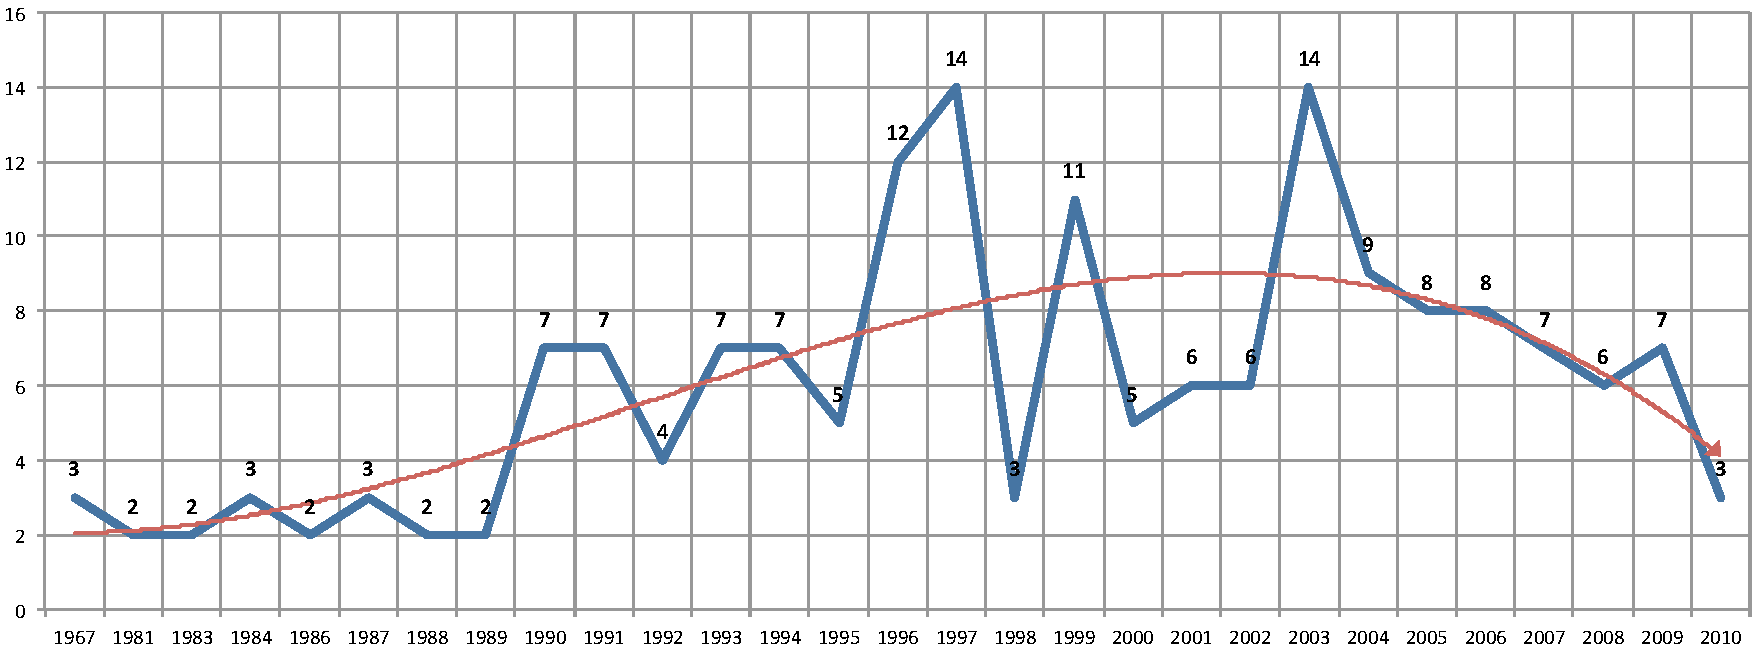
\includegraphics[scale=0.5]{abntex2-modelo-img-grafico.pdf}
	\end{center}
	\legend{Fonte: \citeonline[p. 24]{araujo2012}}
\end{figure}

% ---
\subsection{Figuras em \emph{minipages}}
% ---

\emph{Minipages} são usadas para inserir textos ou outros elementos em quadros
com tamanhos e posições controladas. Veja o exemplo da
\autoref{fig_minipage_imagem1} e da \autoref{fig_minipage_grafico2}.

\begin{figure}[htb]
 \label{teste}
 \centering
  \begin{minipage}{0.4\textwidth}
    \centering
    \caption{Imagem 1 da minipage} \label{fig_minipage_imagem1}
    
\includegraphics[scale=0.9]{abntex2-modelo-img-marca.pdf}
    \legend{Fonte: Produzido pelos autores}
  \end{minipage}
  \hfill
  \begin{minipage}{0.4\textwidth}
    \centering
    \caption{Grafico 2 da minipage} \label{fig_minipage_grafico2}
    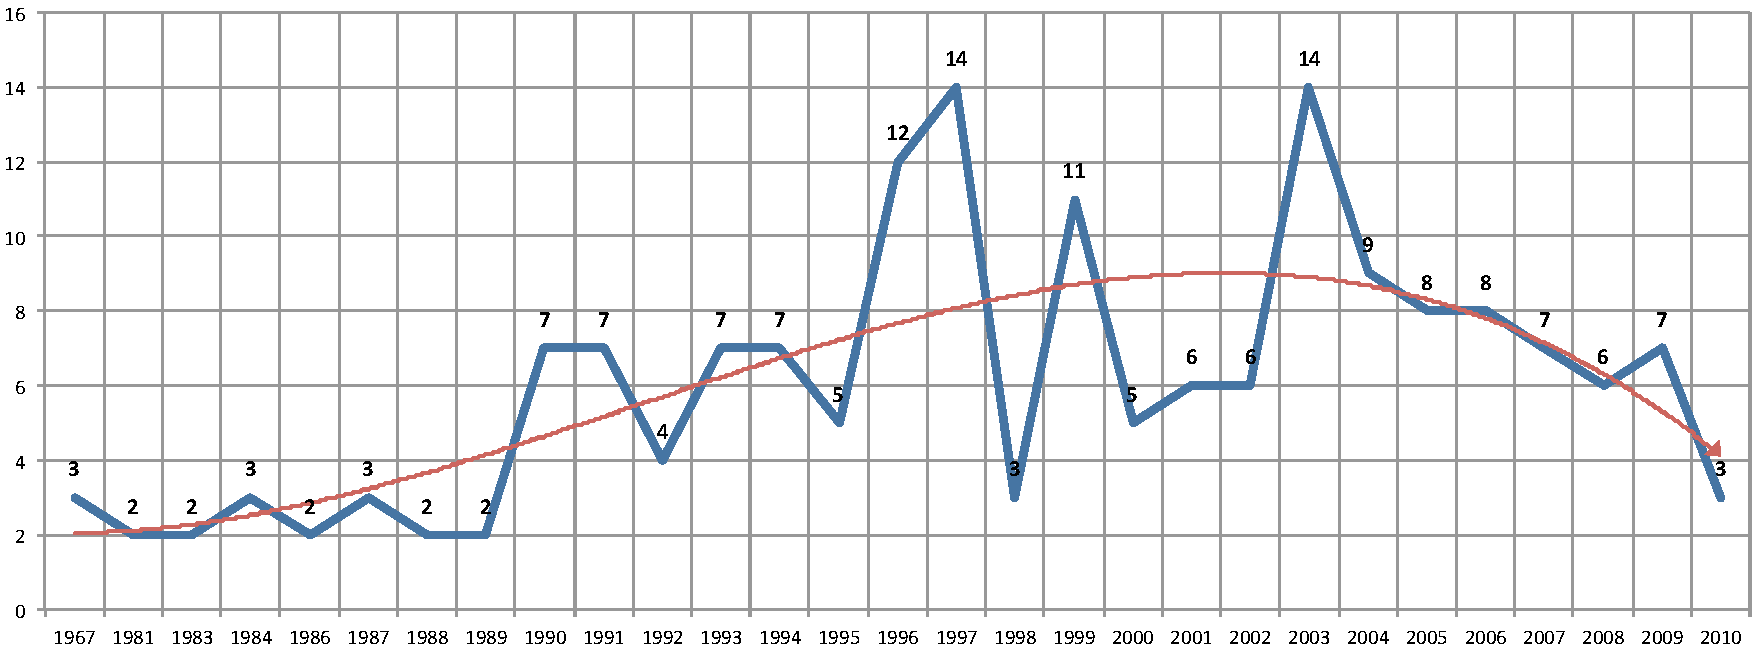
\includegraphics[scale=0.2]{abntex2-modelo-img-grafico.pdf}
    \legend{Fonte: \citeonline[p. 24]{araujo2012}}
  \end{minipage}
\end{figure}

Observe que, segundo a \citeonline[seções 4.2.1.10 e 5.8]{NBR14724:2011}, as
ilustrações devem sempre ter numeração contínua e única em todo o documento:

\begin{citacao}
Qualquer que seja o tipo de ilustração, sua identificação aparece na parte
superior, precedida da palavra designativa (desenho, esquema, fluxograma,
fotografia, gráfico, mapa, organograma, planta, quadro, retrato, figura,
imagem, entre outros), seguida de seu número de ordem de ocorrência no texto,
em algarismos arábicos, travessão e do respectivo título. Após a ilustração, na
parte inferior, indicar a fonte consultada (elemento obrigatório, mesmo que
seja produção do próprio autor), legenda, notas e outras informações
necessárias à sua compreensão (se houver). A ilustração deve ser citada no
texto e inserida o mais próximo possível do trecho a que se
refere. \cite[seções 5.8]{NBR14724:2011}
\end{citacao}

% ---
\section{Expressões matemáticas}
% ---

\index{expressões matemáticas}Use o ambiente \texttt{equation} para escrever
expressões matemáticas numeradas:

\begin{equation}
  \forall x \in X, \quad \exists \: y \leq \epsilon
\end{equation}

Escreva expressões matemáticas entre \$ e \$, como em $ \lim_{x \to \infty}
\exp(-x) = 0 $, para que fiquem na mesma linha.

Também é possível usar colchetes para indicar o início de uma expressão
matemática que não é numerada.

\[
\left|\sum_{i=1}^n a_ib_i\right|
\le
\left(\sum_{i=1}^n a_i^2\right)^{1/2}
\left(\sum_{i=1}^n b_i^2\right)^{1/2}
\]

Consulte mais informações sobre expressões matemáticas em
\url{https://github.com/abntex/abntex2/wiki/Referencias}.

% ---
\section{Enumerações: alíneas e subalíneas}
% ---

\index{alíneas}\index{subalíneas}\index{incisos}Quando for necessário enumerar
os diversos assuntos de uma seção que não possua título, esta deve ser
subdividida em alíneas \cite[4.2]{NBR6024:2012}:

\begin{alineas}

  \item os diversos assuntos que não possuam título próprio, dentro de uma mesma
  seção, devem ser subdivididos em alíneas; 
  
  \item o texto que antecede as alíneas termina em dois pontos;
  \item as alíneas devem ser indicadas alfabeticamente, em letra minúscula,
  seguida de parêntese. Utilizam-se letras dobradas, quando esgotadas as
  letras do alfabeto;

  \item as letras indicativas das alíneas devem apresentar recuo em relação à
  margem esquerda;

  \item o texto da alínea deve começar por letra minúscula e terminar em
  ponto-e-vírgula, exceto a última alínea que termina em ponto final;

  \item o texto da alínea deve terminar em dois pontos, se houver subalínea;

  \item a segunda e as seguintes linhas do texto da alínea começa sob a
  primeira letra do texto da própria alínea;
  
  \item subalíneas \cite[4.3]{NBR6024:2012} devem ser conforme as alíneas a
  seguir:

  \begin{alineas}
     \item as subalíneas devem começar por travessão seguido de espaço;

     \item as subalíneas devem apresentar recuo em relação à alínea;

     \item o texto da subalínea deve começar por letra minúscula e terminar em
     ponto-e-vírgula. A última subalínea deve terminar em ponto final, se não
     houver alínea subsequente;

     \item a segunda e as seguintes linhas do texto da subalínea começam sob a
     primeira letra do texto da própria subalínea.
  \end{alineas}
  
  \item no \abnTeX\ estão disponíveis os ambientes \texttt{incisos} e
  \texttt{subalineas}, que em suma são o mesmo que se criar outro nível de
  \texttt{alineas}, como nos exemplos à seguir:
  
  \begin{incisos}
    \item \textit{Um novo inciso em itálico};
  \end{incisos}
  
  \item Alínea em \textbf{negrito}:
  
  \begin{subalineas}
    \item \textit{Uma subalínea em itálico};
    \item \underline{\textit{Uma subalínea em itálico e sublinhado}}; 
  \end{subalineas}
  
  \item Última alínea com \emph{ênfase}.
  
\end{alineas}

% ---
\section{Espaçamento entre parágrafos e linhas}
% ---

\index{espaçamento!dos parágrafos}O tamanho do parágrafo, espaço entre a margem
e o início da frase do parágrafo, é definido por:

\begin{verbatim}
   \setlength{\parindent}{1.3cm}
\end{verbatim}

\index{espaçamento!do primeiro parágrafo}Por padrão, não há espaçamento no
primeiro parágrafo de cada início de divisão do documento
(\autoref{sec-divisoes}). Porém, você pode definir que o primeiro parágrafo
também seja indentado, como é o caso deste documento. Para isso, apenas inclua o
pacote \textsf{indentfirst} no preâmbulo do documento:

\begin{verbatim}
   \usepackage{indentfirst}      % Indenta o primeiro parágrafo de cada seção.
\end{verbatim}

\index{espaçamento!entre os parágrafos}O espaçamento entre um parágrafo e outro
pode ser controlado por meio do comando:

\begin{verbatim}
  \setlength{\parskip}{0.2cm}  % tente também \onelineskip
\end{verbatim}

\index{espaçamento!entre as linhas}O controle do espaçamento entre linhas é
definido por:

\begin{verbatim}
  \OnehalfSpacing       % espaçamento um e meio (padrão); 
  \DoubleSpacing        % espaçamento duplo
  \SingleSpacing        % espaçamento simples	
\end{verbatim}

Para isso, também estão disponíveis os ambientes:

\begin{verbatim}
  \begin{SingleSpace} ...\end{SingleSpace}
  \begin{Spacing}{hfactori} ... \end{Spacing}
  \begin{OnehalfSpace} ... \end{OnehalfSpace}
  \begin{OnehalfSpace*} ... \end{OnehalfSpace*}
  \begin{DoubleSpace} ... \end{DoubleSpace}
  \begin{DoubleSpace*} ... \end{DoubleSpace*} 
\end{verbatim}

Para mais informações, consulte \citeonline[p. 47-52 e 135]{memoir}.

% ---
\section{Inclusão de outros arquivos}\label{sec-include}
% ---

É uma boa prática dividir o seu documento em diversos arquivos, e não
apenas escrever tudo em um único. Esse recurso foi utilizado neste
documento. Para incluir diferentes arquivos em um arquivo principal,
de modo que cada arquivo incluído fique em uma página diferente, utilize o
comando:

\begin{verbatim}
   \include{documento-a-ser-incluido}      % sem a extensão .tex
\end{verbatim}

Para incluir documentos sem quebra de páginas, utilize:

\begin{verbatim}
   \input{documento-a-ser-incluido}      % sem a extensão .tex
\end{verbatim}

% ---
\section{Compilar o documento \LaTeX}
% ---

Geralmente os editores \LaTeX, como o
TeXlipse\footnote{\url{http://texlipse.sourceforge.net/}}, o
Texmaker\footnote{\url{http://www.xm1math.net/texmaker/}}, entre outros,
compilam os documentos automaticamente, de modo que você não precisa se
preocupar com isso.

No entanto, você pode compilar os documentos \LaTeX usando os seguintes
comandos, que devem ser digitados no \emph{Prompt de Comandos} do Windows ou no
\emph{Terminal} do Mac ou do Linux:

\begin{verbatim}
   pdflatex ARQUIVO_PRINCIPAL.tex
   bibtex ARQUIVO_PRINCIPAL.aux
   makeindex ARQUIVO_PRINCIPAL.idx 
   makeindex ARQUIVO_PRINCIPAL.nlo -s nomencl.ist -o ARQUIVO_PRINCIPAL.nls
   pdflatex ARQUIVO_PRINCIPAL.tex
   pdflatex ARQUIVO_PRINCIPAL.tex
\end{verbatim}

% ---
\section{Remissões internas}
% ---

Ao nomear a \autoref{tab-nivinv} e a \autoref{fig_circulo}, apresentamos um
exemplo de remissão interna, que também pode ser feita quando indicamos o
\autoref{cap_exemplos}, que tem o nome \emph{\nameref{cap_exemplos}}. O número
do capítulo indicado é \ref{cap_exemplos}, que se inicia à
\autopageref{cap_exemplos}\footnote{O número da página de uma remissão pode ser
obtida também assim:
\pageref{cap_exemplos}.}.
Veja a \autoref{sec-divisoes} para outros exemplos de remissões internas entre
seções, subseções e subsubseções.

O código usado para produzir o texto desta seção é:

\begin{verbatim}
Ao nomear a \autoref{tab-nivinv} e a \autoref{fig_circulo}, apresentamos um
exemplo de remissão interna, que também pode ser feita quando indicamos o
\autoref{cap_exemplos}, que tem o nome \emph{\nameref{cap_exemplos}}. O número
do capítulo indicado é \ref{cap_exemplos}, que se inicia à
\autopageref{cap_exemplos}\footnote{O número da página de uma remissão pode ser
obtida também assim:
\pageref{cap_exemplos}.}.
Veja a \autoref{sec-divisoes} para outros exemplos de remissões internas entre
seções, subseções e subsubseções.
\end{verbatim}

% ---
\section{Divisões do documento: seção}\label{sec-divisoes}
% ---

Esta seção testa o uso de divisões de documentos. Esta é a
\autoref{sec-divisoes}. Veja a \autoref{sec-divisoes-subsection}.

\subsection{Divisões do documento: subseção}\label{sec-divisoes-subsection}

Isto é uma subseção. Veja a \autoref{sec-divisoes-subsubsection}, que é uma
\texttt{subsubsection} do \LaTeX, mas é impressa chamada de ``subseção'' porque
no Português não temos a palavra ``subsubseção''.

\subsubsection{Divisões do documento: subsubseção}
\label{sec-divisoes-subsubsection}

Isto é uma subsubseção.

\subsubsection{Divisões do documento: subsubseção}

Isto é outra subsubseção.

\subsection{Divisões do documento: subseção}\label{sec-exemplo-subsec}

Isto é uma subseção.

\subsubsection{Divisões do documento: subsubseção}

Isto é mais uma subsubseção da \autoref{sec-exemplo-subsec}.


\subsubsubsection{Esta é uma subseção de quinto
nível}\label{sec-exemplo-subsubsubsection}

Esta é uma seção de quinto nível. Ela é produzida com o seguinte comando:

\begin{verbatim}
\subsubsubsection{Esta é uma subseção de quinto
nível}\label{sec-exemplo-subsubsubsection}
\end{verbatim}

\subsubsubsection{Esta é outra subseção de quinto nível}\label{sec-exemplo-subsubsubsection-outro}

Esta é outra seção de quinto nível.


\paragraph{Este é um parágrafo numerado}\label{sec-exemplo-paragrafo}

Este é um exemplo de parágrafo nomeado. Ele é produzida com o comando de
parágrafo:

\begin{verbatim}
\paragraph{Este é um parágrafo nomeado}\label{sec-exemplo-paragrafo}
\end{verbatim}

A numeração entre parágrafos numeradaos e subsubsubseções são contínuas.

\paragraph{Esta é outro parágrafo numerado}\label{sec-exemplo-paragrafo-outro}

Esta é outro parágrafo nomeado.

% ---
\section{Este é um exemplo de nome de seção longo. Ele deve estar
alinhado à esquerda e a segunda e demais linhas devem iniciar logo abaixo da
primeira palavra da primeira linha}
% ---

Isso atende à norma \citeonline[seções de 5.2.2 a 5.2.4]{NBR14724:2011} 
 e \citeonline[seções de 3.1 a 3.8]{NBR6024:2012}.

% ---
\section{Diferentes idiomas e hifenizações}
\label{sec-hifenizacao}
% ---

Para usar hifenizações de diferentes idiomas, inclua nas opções do documento o
nome dos idiomas que o seu texto contém. Por exemplo (para melhor
visualização, as opções foram quebras em diferentes linhas):

\begin{verbatim}
\documentclass[
	12pt,
	openright,
	twoside,
	a4paper,
	english,
	french,
	spanish,
	brazil
	]{abntex2}
\end{verbatim}

O idioma português-brasileiro (\texttt{brazil}) é incluído automaticamente pela
classe \textsf{abntex2}. Porém, mesmo assim a opção \texttt{brazil} deve ser
informada como a última opção da classe para que todos os pacotes reconheçam o
idioma. Vale ressaltar que a última opção de idioma é a utilizada por padrão no
documento. Desse modo, caso deseje escrever um texto em inglês que tenha
citações em português e em francês, você deveria usar o preâmbulo como abaixo:

\begin{verbatim}
\documentclass[
	12pt,
	openright,
	twoside,
	a4paper,
	french,
	brazil,
	english
	]{abntex2}
\end{verbatim}

A lista completa de idiomas suportados, bem como outras opções de hifenização,
estão disponíveis em \citeonline[p.~5-6]{babel}.

Exemplo de hifenização em inglês\footnote{Extraído de:
\url{http://en.wikibooks.org/wiki/LaTeX/Internationalization}}:

\begin{otherlanguage*}{english}
\textit{Text in English language. This environment switches all language-related
definitions, like the language specific names for figures, tables etc. to the other
language. The starred version of this environment typesets the main text
according to the rules of the other language, but keeps the language specific
string for ancillary things like figures, in the main language of the document.
The environment hyphenrules switches only the hyphenation patterns used; it can
also be used to disallow hyphenation by using the language name
`nohyphenation'.}
\end{otherlanguage*}

Exemplo de hifenização em francês\footnote{Extraído de:
\url{http://bigbrowser.blog.lemonde.fr/2013/02/17/tu-ne-tweeteras-point-le-vatican-interdit-aux-cardinaux-de-tweeter-pendant-le-conclave/}}:

\begin{otherlanguage*}{french}
\textit{Texte en français. Pas question que Twitter ne vienne faire une
concurrence déloyale à la traditionnelle fumée blanche qui marque l'élection
d'un nouveau pape. Pour éviter toute fuite précoce, le Vatican a donc pris un
peu d'avance, et a déjà interdit aux cardinaux qui prendront part au vote
d'utiliser le réseau social, selon Catholic News Service. Une mesure valable
surtout pour les neuf cardinaux – sur les 117 du conclave – pratiquants très
actifs de Twitter, qui auront interdiction pendant toute la période de se
connecter à leur compte.}
\end{otherlanguage*}

Pequeno texto em espanhol\footnote{Extraído de:
\url{http://internacional.elpais.com/internacional/2013/02/17/actualidad/1361102009_913423.html}}:

\foreignlanguage{spanish}{\textit{Decenas de miles de personas ovacionan al pontífice en su
penúltimo ángelus dominical, el primero desde que anunciase su renuncia. El Papa se
centra en la crítica al materialismo}}.

O idioma geral do texto por ser alterado como no exemplo seguinte:

\begin{verbatim}
  \selectlanguage{english}
\end{verbatim}

Isso altera automaticamente a hifenização e todos os nomes constantes de
referências do documento para o idioma inglês. Consulte o manual da classe
\cite{abntex2classe} para obter orientações adicionais sobre internacionalização de
documentos produzidos com \abnTeX.

A \autoref{sec-citacao} descreve o ambiente \texttt{citacao} que pode receber
como parâmetro um idioma a ser usado na citação.

% ---
\section{Consulte o manual da classe \textsf{abntex2}}
% ---

Consulte o manual da classe \textsf{abntex2} \cite{abntex2classe} para uma
referência completa das macros e ambientes disponíveis. 

Além disso, o manual possui informações adicionais sobre as normas ABNT
observadas pelo \abnTeX\ e considerações sobre eventuais requisitos específicos
não atendidos, como o caso da \citeonline[seção 5.2.2]{NBR14724:2011}, que
especifica o espaçamento entre os capítulos e o início do texto, regra
propositalmente não atendida pelo presente modelo.

% ---
\section{Referências bibliográficas}
% ---

A formatação das referências bibliográficas conforme as regras da ABNT são um
dos principais objetivos do \abnTeX. Consulte os manuais
\citeonline{abntex2cite} e \citeonline{abntex2cite-alf} para obter informações
sobre como utilizar as referências bibliográficas.

%-
\subsection{Acentuação de referências bibliográficas}
%-

Normalmente não há problemas em usar caracteres acentuados em arquivos
bibliográficos (\texttt{*.bib}). Porém, como as regras da ABNT fazem uso quase
abusivo da conversão para letras maiúsculas, é preciso observar o modo como se
escreve os nomes dos autores. Na ~\autoref{tabela-acentos} você encontra alguns
exemplos das conversões mais importantes. Preste atenção especial para `ç' e `í'
que devem estar envoltos em chaves. A regra geral é sempre usar a acentuação
neste modo quando houver conversão para letras maiúsculas.

\begin{table}[htbp]
\caption{Tabela de conversão de acentuação.}
\label{tabela-acentos}

\begin{center}
\begin{tabular}{ll}\hline\hline
acento & \textsf{bibtex}\\
à á ã & \verb+\`a+ \verb+\'a+ \verb+\~a+\\
í & \verb+{\'\i}+\\
ç & \verb+{\c c}+\\
\hline\hline
\end{tabular}
\end{center}
\end{table}


% ---
\section{Precisa de ajuda?}
% ---

Consulte a FAQ com perguntas frequentes e comuns no portal do \abnTeX:
\url{https://github.com/abntex/abntex2/wiki/FAQ}.

Inscreva-se no grupo de usuários \LaTeX:
\url{http://groups.google.com/group/latex-br}, tire suas dúvidas e ajude
outros usuários.

Participe também do grupo de desenvolvedores do \abnTeX:
\url{http://groups.google.com/group/abntex2} e faça sua contribuição à
ferramenta.

% ---
\section{Você pode ajudar?}
% ---

Sua contribuição é muito importante! Você pode ajudar na divulgação, no
desenvolvimento e de várias outras formas. Veja como contribuir com o \abnTeX\
em \url{https://github.com/abntex/abntex2/wiki/Como-Contribuir}.

% ---
\section{Quer customizar os modelos do \abnTeX\ para sua instituição ou
universidade?}
% ---

Veja como customizar o \abnTeX\ em:
\url{https://github.com/abntex/abntex2/wiki/ComoCustomizar}.


% ---

% ----------------------------------------------------------
% PARTE
% ----------------------------------------------------------
\part{Literature Review}
% ----------------------------------------------------------
%% abtex2-modelo-include-comandos.tex, v-1.9.5 laurocesar
%% Copyright 2012-2015 by abnTeX2 group at http://www.abntex.net.br/ 
%%
%% This work may be distributed and/or modified under the
%% conditions of the LaTeX Project Public License, either version 1.3
%% of this license or (at your option) any later version.
%% The latest version of this license is in
%%   http://www.latex-project.org/lppl.txt
%% and version 1.3 or later is part of all distributions of LaTeX
%% version 2005/12/01 or later.
%%
%% This work has the LPPL maintenance status `maintained'.
%% 
%% The Current Maintainer of this work is the abnTeX2 team, led
%% by Lauro César Araujo. Further information are available on 
%% http://www.abntex.net.br/
%%
%% This work consists of the files abntex2-modelo-include-comandos.tex
%% and abntex2-modelo-img-marca.pdf
%%

% ---
% Este capítulo, utilizado por diferentes exemplos do abnTeX2, ilustra o uso de
% comandos do abnTeX2 e de LaTeX.
% ---
 
\chapter{Background}\label{background}
\chapterprecis{The purpose of this section is to understand the problem.}\index{sinopse de capítulo}

% ---
\section{Similar Selection Systems}
% ---

\noindent
An optimization procedure which is similar to ours is presented by \cite{raynersss13}, but their procedure maximizes the average heuristic value. By contrast, the meta$-$reasoning we are proposing minimizes the search tree size.\\

Our meta$-$reasoning requires a prediction of the number of nodes expanded by A$\sp{*}$ using any given subset. Although there are methods for accurately predicting the number of nodes expanded by Iterative Deepening$-$A$\sp{*}$ \cite{Korf85ida} (ID$A\sp{*}$). (\texttt{SS} system  \cite{lelis2013predicting}), these methods can't be easily adapted to A$\sp{*}$ because A$\sp{*}$'s duplicate pruning makes it very difficult to predict how many nodes will occur at depth $d$ of $A\sp{*}$'s search tree (the tree of nodes expanded by $A\sp{*}$). As a part of our proposal, we present \texttt{SS} for predicting the size of the search tree.

The system most similar to ours is \textbf{RIDA$\sp{*}$} \cite{BarleySantiagoOver}. \textbf{RIDA$\sp{*}$} also selects a subset from a pool of heuristics to guide the $A\sp{*}$ search. In \textbf{RIDA$\sp{*}$} this is done by starting with an empty subset and trying all combination of size one before trying the combination of size two and so on. \textbf{RIDA$\sp{*}$} stops after evaluating a fixed number of subsets. While \textbf{RIDA$\sp{*}$} is able to evaluate a set of heuristics with tens of elements, our meta$-$reasoning is able to evaluate a set of heuristics with thousands of elements.

% ---
\section{Problem definition}
% ---

A $SAS\sp{+} planning\ task$ \cite{backstrom1995complexity} is a 4 tuple $\triangledown = \{V, O, I, G\}.$ \textit{V} is a set of \textit{state variables.} Each variable \textit{v} $\in$ \textit{V} is associated with a finite domain of possible $D_{\substack{v}}$. A state is an assignment of a value to every $v \in V.$ The set of possible states, denoted \textit{V}, is therefore $D_{\substack{v_{\substack{1}}}}    \times ... \times D_{\substack{v_{\substack{2}}}}$. \textit{O} is a set of operators, where each operator $o \in O$ is triple $\{pre_{\substack{o}} , post_{\substack{o}}, cost_{\substack{o}}\}$ specifying the preconditions, postconditions (effects), and non-negative cost of \textit{o}. $pre_{\substack{o}}\ and\ post_{\substack{o}}$ are assignments of values to subsets os variables, $V_{\substack{pre_{\substack{o}}}}\ and\ V_{\substack{post_{\substack{o}}}}$, respectively. Operator \textit{o} is applicable to state \textit{s} if \textit{s} and $pre_{\substack{o}}$ agree on the assignment of values to variables in $V_{\substack{pre_{\substack{o}}}}$. The effect of \textit{o}, when applied to \textit{s}, is to set the variables in $V_{\substack{post_{\substack{o}}}}$ to the values specified in $post_{\substack{o}}$ and to set all other variables to the value they have in \textit{s}. \textit{G} is the goal condition, an assignment of values to a subset of variables, $V_{\substack{G}}$. A state is a goal state if it and \textit{G} agree on the assignment of values to the variable in $V_{\substack{G}}$. \textit{I} is the initial state, and the planning task, $\triangledown$, is to find an optimal (least-cost) sequence of operators leading from \textit{I} to a goal state. We denote the optimal solution cost of $\triangledown$ as $C\sp{*}$ \\

The state space problem illustrated in the figure \ref{fig:8tilepuzzle_begin} is a game that consists of a frame of numbered square tiles in random order with one tile missing. The puzzle also exists in other sizes, particularly the smaller 8$-$puzzle. If the size is 3$\times$3 tiles, the puzzle is called the 8$-$puzzle or 9$-$puzzle, and if 4 $\times$ 4 tiles, the puzzle is called the 15$-$puzzle or 16$-$puzzle named, respectively, for the number of tiles and the number of spaces. The object of the puzzle is to place the tiles in order by making sliding moves that use the empty space. \\

The legal operators are to slide any tile that is horizontally or vertically adjacent to the blank into the blank position. The problem is to rearrange the tiles from some random initial configuration into a particular desired goal configuration. The 8$-$puzzle contains 181,440 reachable states, the 15$-$puzzle contains about $10\sp{13}$ reachable states, and the 24$-$puzzle contains almost $10\sp{25}$ states. \\

\begin{figure}[htb]
\centering
\begin{forest}
 [\usebox\myboxa \hspace*{1.4in} \usebox\myboxb]
 $\node [xshift=-5.5cm,yshift=3.5cm] (A) at (2,0) {Initial};$
 $\node [xshift=1.5cm,yshift=3.5cm] (A) at (2,0) {Goal};$
\end{forest}
\caption{The left tile$-$puzzle is the initial distribution of tiles and the right tile$-$puzzle is the goal distribution of tiles. Each one represent a State.} \label{fig:8tilepuzzle_begin}
\end{figure}


Instead of using an algorithm of Brute force search that will analyze all the possible solutions. We can obtain heuristics from the problem of the slide tile puzzle that will help us to solve the problem.

\section{Heuristics}
State$-$space algorithms, such as A* \cite{hart1968formal}, are important in many \texttt{AI} applications. A* uses the $f(s) = g(s) + h(s)$ cost function to guide its search. Here, $g(s)$ is the cost of the path from the start state $s$, and $h(s)$ is the estimated cost$-$to$-$go from $s$ to a gial; $h(.)$ is known as the heuristic function. The heuristic is the mathematical concept that represent to the estimate distance from the node $s$ to the nearest goal state.

\begin{figure}[htb]
\centering
\begin{tikzpicture}
	%\draw[yshift=-1 em, ultra thick] (0,0) [point] -- (5,0) [point] -- (10,0) [point];
	\coordinate (I) at (0,0) (I) node[point=ultra thick, above] {I};
	\coordinate (I1) at (2,0) (I1) node[point=ultra thick, above] {};
	\coordinate (I2) at (4,0) (I2) node[point=ultra thick, above] {};
	\coordinate (I3) at (6,0) (I3) node[point=ultra thick, above] {};
	\coordinate (s) at (8,0) (s) node[point=ultra thick, above] {s};
	\coordinate (I4) at (10,0) (I4) node[point=ultra thick, above] {};
	\coordinate (I5) at (12,0) (I5) node[point=ultra thick, above] {};
	\coordinate (G) at (14,0) (G) node[point=ultra thick, above] {G};
	\draw (I) -- (G);	

\draw [decorate,decoration={brace,amplitude=4pt},xshift=4pt,yshift=14pt]
(8,0) -- (12,0) node [black,midway,yshift=0.5cm] 
{\footnotesize $h(s)=2$};

\draw [decorate,decoration={brace,amplitude=8pt,mirror},xshift=4pt,yshift=-14pt]
(0,0) -- (8,0) node [black,midway,yshift=-0.5cm] 
{\footnotesize $g(s)=4$};


\draw [decorate,decoration={brace,amplitude=6pt,mirror},xshift=4pt,yshift=-14pt]
(8,0) -- (14,0) node [black,midway,yshift=-0.5cm] 
{\footnotesize $h\sp{*}(s)=3$};
\end{tikzpicture}
\caption{Heuristic Search: \textit{I}: Initial State, \textit{s}: Some Sate, \textit{G}: Goal State} \label{fig:searchSpace}
\end{figure}

In the figure \ref{fig:searchSpace} the optimal distance from the Initial State $I$ to  the state $s$ is 4 and represented by $g(s)$. The $h\sp{*}(s)$ represent the optimal distance from $s$ to the Goal State $G$. And the $h(s)$ is the estimation distance from $s$ to $G$.

A heuristic function $h(s)$ estimates the cost of a solution path from $s$ to a goal state. A heuristic is admissible if $h(s) \leq h\sp{*}(s)$ for all $s \in V$, where $h\sp{*}(s)$ is the optimal cost of $s$. A heuristic is consisten iff $h(s) \leq c(s,t) + h(t)$ for all states $s$ and $t$, where $c(s,t)$ is the cost of the cheapest path from $s$ to $t$. For example, the heuristic function provided by a pattern database (\texttt{PDB}) heuristic \cite{culberson1998pattern} is admissible and consistent.

Given a set of admissible and consistent heuristics $\zeta = \{h_{1}, h_{2}, \dots, h_{M}\}$, the heuristic $h_{max}(s,\zeta) = $max$_{h \in \zeta} h(s)$ is also admissible and consistent. When describing our method we assume all heuristics to be consistent. We define $f_{max}(s, \zeta) = g(s) + h_{max}(s, \zeta)$, where $g(s)$ is the cost of the path expanded from $I$ to $s$. $g(s)$ is minimal when A$\sp{*}$ using a consistent heuristic expands $s$. We call an A$\sp{*}$ search tree the tree defined by the states expanded by A$\sp{*}$ using a consistent heuristic while solving a problem $\triangledown$.

The heuristics can be obtained from each state of the problem. For example, for the problem of the 8$-$tile$-$puzzle figure \ref{fig:8tilepuzzle_begin} we can get two heuristics.

\subsection{Out of place (O.P)}
Counts the number of objects out of place.

\begin{figure}[htb]
\centering
\begin{forest}
 [\usebox\myboxa]
 $\draw[->,xshift=4pt,yshift=14pt] (2,1) -- (4,1);$
 $\node [xshift=1cm,yshift=2cm] (A) at (2,0) {O.P=8};$
 \hspace*{1.8in} 
 %$\rightarrow$  
 [\usebox\myboxb] 
\end{forest}
\caption{Out of place heuristic} \label{fig:8tilepuzzle_oop}
\end{figure}

The tiles numbered with 4, 1, 2, 3, 6, 7, 5, 8, and 4 are out of place then each object count as 1 and the sum would be 8.

\subsection{Manhatham Distance (M.D)}
Counts the minimum number of operations to get to the goal state.

\begin{figure}[htb]
\centering
\begin{forest}
 [\usebox\myboxa]
 $\draw[->,xshift=4pt,yshift=14pt] (2,1) -- (4,1);$
 $\node [xshift=1cm,yshift=2cm] (A) at (2,0) {M.D=1O};$
 \hspace*{1.8in} 
 %$\rightarrow$  
 [\usebox\myboxb] 
\end{forest}
\caption{Manhatham distance heuristic} \label{fig:8tilepuzzle_md}
\end{figure}

The tile 4 count 1 to get to the goal position.
The tile 1 count 1 to get to the goal position.
The tile 2 count 1 to get to the goal position.
The tile 3 count 1 to get to the goal position.
The tile 6 count 1 to get to the goal position.
The tile 7 count 1 to get to the goal position.
The tile 5 count 1 to get to the goal position.
The tile 8 count 1 to get to the goal position.
Then the sum would be 10.

In order to solve the problem, we get the heuristics, which are information from the problem to solve the problem. Exists systems that can create heuristics for each problem. Those systems are called Heuristic Generators.

\section{Heuristic Generators}
Heuristic Generators works by creating abstractions of the original problem space. The approach that has showed more successful results lately is \texttt{PDB}.

\subsection{Pattern Database (PDB)}
It's obtained by abstracting away certain problem variables, so that the remaining problem ("pattern") is small enough to be solved optimally for every state by blind exhaustive search. The results stored in a table, represent a PDB for the original problem. The abstraction of the search space gives an admissible heuristic function, mapping states to lower bounds.

\section{Take advantage of Heuristics}
The heuristics generators can create hundreds or even thousand of heuristics. In fact, exists different ways to take advantage of those heuristics. For example: If we want to use all the heuristics created by the heuristic generator. It would not be a good idea to use all of them because the main problem involved would be the time to evaluate each heuristic in the search tree, it could take too much time. \\

One way to take advantage of heuristics would be to take the maximum of the set of heuristics. For example, using three different heuristics $h1, h2$ and max($h1, h2$). Heuristic $h1$ and $h2$ are based on domain abstractions and the max($h1, h2$) is the maximum heuristic value of $h1$ and $h2$. \\

Exists different approaches to take advantage from a large set of heuristics. In this dissertation we use the meta$-$reasoning based on the minimum evaluation time. \\


\section{Number of heuristics created}
Let's suppose we have to run our meta$-$reasoning using M amount of memory available. The question would be: How many heuristics our system should handle in order to avoid out of memory errors? So. one of the objectives of this tesis is to find the number of heuristics that our subset $\zeta\sp{'}$ should have.

\begin{figure}[htb]
  \centering
  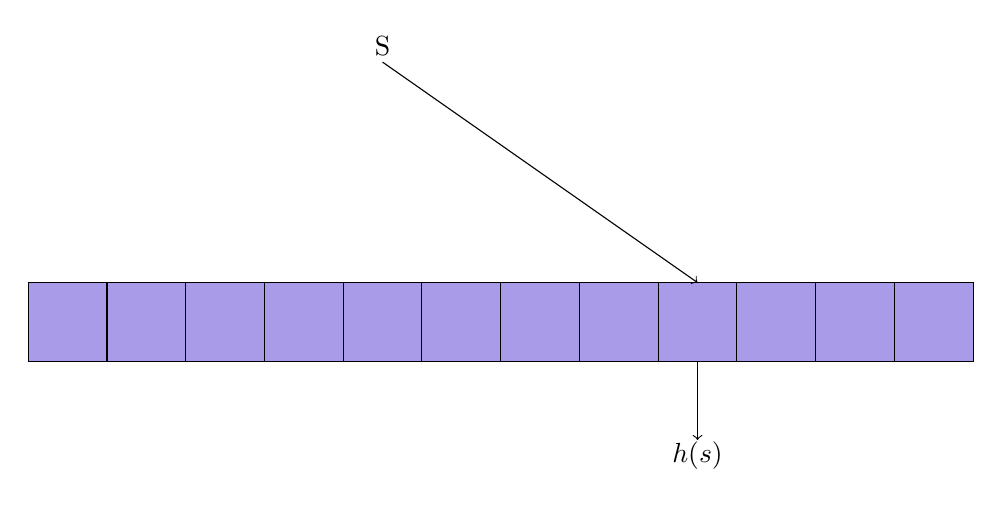
\begin{tikzpicture}
\draw[step=1cm,gray,very thin] grid (12,1);
%\draw[step=1cm,gray,very thin] (-1.9,-1.9) grid (5.9,5.9);
%\fill[blue!40!white] (0,0) rectangle (4,4);
\filldraw[fill=blue!40!white, draw=black] rectangle (12,1);
\filldraw[fill=blue!40!white, draw=black] rectangle (11,1);
\filldraw[fill=blue!40!white, draw=black] rectangle (10,1);
\filldraw[fill=blue!40!white, draw=black] rectangle (9,1);
\filldraw[fill=blue!40!white, draw=black] rectangle (8,1);
\filldraw[fill=blue!40!white, draw=black] rectangle (7,1);
\filldraw[fill=blue!40!white, draw=black] rectangle (6,1);
\filldraw[fill=blue!40!white, draw=black] rectangle (5,1);
\filldraw[fill=blue!40!white, draw=black] rectangle (4,1);
\filldraw[fill=blue!40!white, draw=black] rectangle (3,1);
\filldraw[fill=blue!40!white, draw=black] rectangle (2,1);
\filldraw[fill=blue!40!white, draw=black] rectangle (1,1);

 %$\draw[->,xshift=4pt,yshift=14pt] (2,1) -- (4,1);$
 \node [xshift=2.5cm,yshift=4cm] (A) at (2,0) {S};
 
 %\draw[->] (2.5cm,8em) -- (8cm,5em) node[midway,right] {\Om{2}};
 \draw[->] (4.5,3.8) -- (8.5,1) node[midway,right] {\Vpi{}};
 \draw[->] (8.5,0) -- (8.5,-1) node[xshift=0cm,yshift=-0.2cm] {$h(s)$};
\end{tikzpicture}
  \caption{One heuristic of size M}\label{fig:image1mem}
\end{figure}

\begin{figure}[htb]
  \centering
  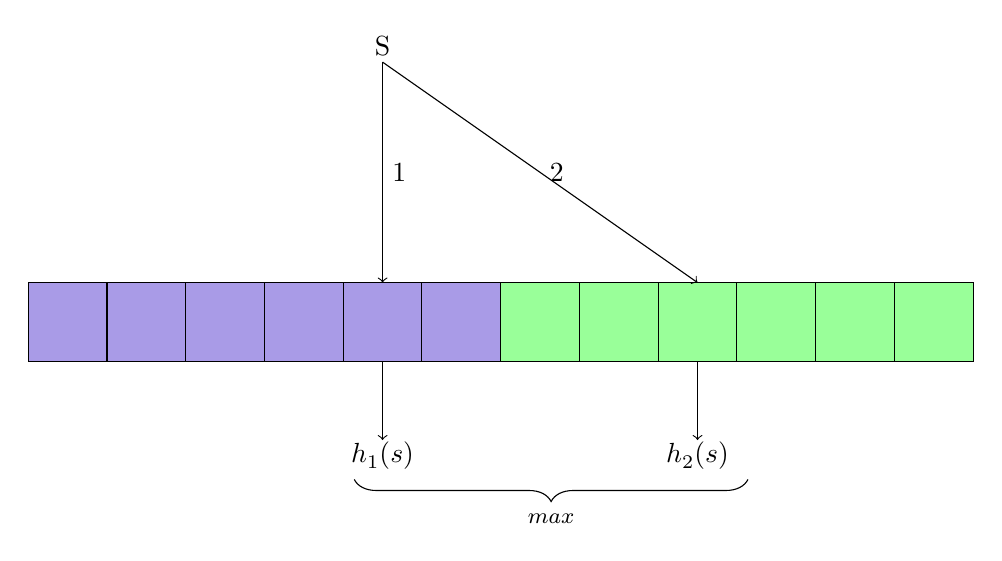
\begin{tikzpicture}
\draw[step=1cm,gray,very thin] grid (12,1);
%\draw[step=1cm,gray,very thin] (-1.9,-1.9) grid (5.9,5.9);
%\fill[blue!40!white] (0,0) rectangle (4,4);
\filldraw[fill=green!40!white, draw=black] rectangle (12,1);
\filldraw[fill=green!40!white, draw=black] rectangle (11,1);
\filldraw[fill=green!40!white, draw=black] rectangle (10,1);
\filldraw[fill=green!40!white, draw=black] rectangle (9,1);
\filldraw[fill=green!40!white, draw=black] rectangle (8,1);
\filldraw[fill=green!40!white, draw=black] rectangle (7,1);
\filldraw[fill=blue!40!white, draw=black] rectangle (6,1);
\filldraw[fill=blue!40!white, draw=black] rectangle (5,1);
\filldraw[fill=blue!40!white, draw=black] rectangle (4,1);
\filldraw[fill=blue!40!white, draw=black] rectangle (3,1);
\filldraw[fill=blue!40!white, draw=black] rectangle (2,1);
\filldraw[fill=blue!40!white, draw=black] rectangle (1,1);

 %$\draw[->,xshift=4pt,yshift=14pt] (2,1) -- (4,1);$
 \node [xshift=2.5cm,yshift=4cm] (A) at (2,0) {S};
 
 %\draw[->] (2.5cm,8em) -- (8cm,5em) node[midway,right] {\Om{2}};
 \draw[->] (4.5,3.8) -- (4.5,1) node[midway,right] {\Vpi{1}};
 \draw[->] (4.5,0) -- (4.5,-1) node[xshift=0cm,yshift=-0.2cm] {$h_{\substack{1}}(s)$};
 
 \draw[->] (4.5,3.8) -- (8.5,1) node[midway,right] {\Vpi{2}};
 \draw[->] (8.5,0) -- (8.5,-1) node[xshift=0cm,yshift=-0.2cm] {$h_{\substack{2}}(s)$};
 
 \draw[decorate,decoration={brace,amplitude=8pt,mirror},xshift=4pt,yshift=-1.5cm]
(4,0) -- (9,0) node [black,midway,yshift=-0.5cm] 
{\footnotesize $max$};
\end{tikzpicture}
  \caption{Two heuristics of size M/2}\label{fig:image2mem}
\end{figure}

\begin{figure}[htb]
  \centering
  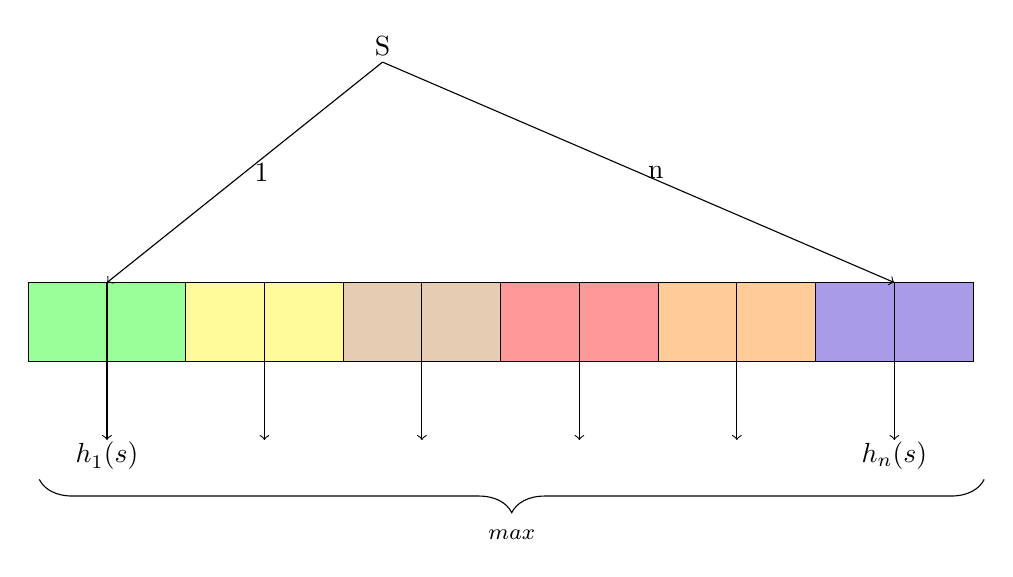
\begin{tikzpicture}
\draw[step=1cm,gray,very thin] grid (12,1);
%\draw[step=1cm,gray,very thin] (-1.9,-1.9) grid (5.9,5.9);
%\fill[blue!40!white] (0,0) rectangle (4,4);
\filldraw[fill=blue!40!white, draw=black] rectangle (12,1);
\filldraw[fill=blue!40!white, draw=black] rectangle (11,1);
\filldraw[fill=orange!40!white, draw=black] rectangle (10,1);
\filldraw[fill=orange!40!white, draw=black] rectangle (9,1);
\filldraw[fill=red!40!white, draw=black] rectangle (8,1);
\filldraw[fill=red!40!white, draw=black] rectangle (7,1);
\filldraw[fill=brown!40!white, draw=black] rectangle (6,1);
\filldraw[fill=brown!40!white, draw=black] rectangle (5,1);
\filldraw[fill=yellow!40!white, draw=black] rectangle (4,1);
\filldraw[fill=yellow!40!white, draw=black] rectangle (3,1);
\filldraw[fill=green!40!white, draw=black] rectangle (2,1);
\filldraw[fill=green!40!white, draw=black] rectangle (1,1);

 %$\draw[->,xshift=4pt,yshift=14pt] (2,1) -- (4,1);$
 \node [xshift=2.5cm,yshift=4cm] (A) at (2,0) {S};

 \draw[->] (4.5,3.8) -- (1,1) node[midway,right] {\Vpi{1}};
 \draw[->] (1,0) -- (1,-1) node[xshift=0cm,yshift=-0.2cm] {$h_{\substack{1}}(s)$};
 
 \draw[->] (4.5,3.8) -- (11,1) node[midway,right] {\Vpi{n}};
 \draw[->] (11,0) -- (11,-1) node[xshift=0cm,yshift=-0.2cm] {$h_{\substack{n}}(s)$};
 
%draw each arrow
\draw[->] (3,0) -- (3,-1) node[xshift=0cm,yshift=-0.2cm] {};
\draw[->] (5,0) -- (5,-1) node[xshift=0cm,yshift=-0.2cm] {};
\draw[->] (7,0) -- (7,-1) node[xshift=0cm,yshift=-0.2cm] {};
\draw[->] (9,0) -- (9,-1) node[xshift=0cm,yshift=-0.2cm] {}; 

 \draw[decorate,decoration={brace,amplitude=12pt,mirror},xshift=4pt,yshift=-1.5cm]
(0,0) -- (12,0) node [black,midway,yshift=-0.7cm] 
{\footnotesize $max$};
\end{tikzpicture}
  \caption{N heuristics of size M/N}\label{fig:image3mem}
\end{figure}

In the Figures \ref{fig:image2mem} and \ref{fig:image3mem} we are taking advantange of the heuristics doing the maximization of all the heuristics created.

\clearpage

\section{Heuristic Subset}
The heuristics generator systems can create a large number of heuristics. Let's suppose $|\zeta| = $ 1000 heuristics were created considering the time and memory avaiable and we want to select the best N $=$ 100 heuristics. This would be: $${1000\choose 100} = 10\sp{138} possibilities$$
So, try to select heuristics from a large set of heuristics are going to be treated as an optimization problem. Then, in order to obtain a good selection of subset of heuristics, our objective function should guarantee two properties: Monotonicity and Submodularity, that would be explained in the next Part. \\
 \bigskip

In the next Part, we will introduce the meta$-$reasoning proposed for selecting heuristics and will expand on the properties of our objective functions.\\

\clearpage
% ---
% Capitulo de revisão de literatura
% ---
%\chapter{Lorem ipsum dolor sit amet}
% ---

% ---
%\section{Aliquam vestibulum fringilla lorem}
% ---

%\lipsum[1]

%\lipsum[2-3]

% ----------------------------------------------------------
% PARTE
% ----------------------------------------------------------
\part{Resultados}
% ----------------------------------------------------------

% ---
% primeiro capitulo de Resultados
% ---
\chapter{Lectus lobortis condimentum}
% ---

% ---
\section{Vestibulum ante ipsum primis in faucibus orci luctus et ultrices
posuere cubilia Curae}
% ---

\lipsum[21-22]

% ---
% segundo capitulo de Resultados
% ---
\chapter{Nam sed tellus sit amet lectus urna ullamcorper tristique interdum
elementum}
% ---

% ---
\section{Pellentesque sit amet pede ac sem eleifend consectetuer}
% ---

\lipsum[24]

% ----------------------------------------------------------
% Finaliza a parte no bookmark do PDF
% para que se inicie o bookmark na raiz
% e adiciona espaço de parte no Sumário
% ----------------------------------------------------------
\phantompart

% ---
% Conclusão
% ---
\chapter{Conclusão}
% ---

\lipsum[31-33]

% ----------------------------------------------------------
% ELEMENTOS PÓS-TEXTUAIS
% ----------------------------------------------------------
\postextual
% ----------------------------------------------------------

% ----------------------------------------------------------
% Referências bibliográficas
% ----------------------------------------------------------
\bibliography{abntex2-modelo-references}

% ----------------------------------------------------------
% Glossário
% ----------------------------------------------------------
%
% Consulte o manual da classe abntex2 para orientações sobre o glossário.
%
%\glossary

% ----------------------------------------------------------
% Apêndices
% ----------------------------------------------------------

% ---
% Inicia os apêndices
% ---
\begin{apendicesenv}

% Imprime uma página indicando o início dos apêndices
\partapendices

% ----------------------------------------------------------
\chapter{Quisque libero justo}
% ----------------------------------------------------------

\lipsum[50]

% ----------------------------------------------------------
\chapter{Nullam elementum urna vel imperdiet sodales elit ipsum pharetra ligula
ac pretium ante justo a nulla curabitur tristique arcu eu metus}
% ----------------------------------------------------------
\lipsum[55-57]

\end{apendicesenv}
% ---


% ----------------------------------------------------------
% Anexos
% ----------------------------------------------------------

% ---
% Inicia os anexos
% ---
\begin{anexosenv}

% Imprime uma página indicando o início dos anexos
\partanexos

% ---
\chapter{Morbi ultrices rutrum lorem.}
% ---
\lipsum[30]

% ---
\chapter{Cras non urna sed feugiat cum sociis natoque penatibus et magnis dis
parturient montes nascetur ridiculus mus}
% ---

\lipsum[31]

% ---
\chapter{Fusce facilisis lacinia dui}
% ---

\lipsum[32]

\end{anexosenv}

%---------------------------------------------------------------------
% INDICE REMISSIVO
%---------------------------------------------------------------------
\phantompart
\printindex
%---------------------------------------------------------------------

\end{document}